\subsection{Banco de atenuadores y aisladores N2002A (Noise Source Test Set )}
El banco de atenuadores y aisladores N2002A (figura \ref{Fig:BancoAtenuadoresAisladores}) es un dispositivo que, de acuerdo a la nota de aplicación de Agilent Technologies \cite{AGI02}, esta destinado a facilitar la calibración de fuentes de ruido de forma rápida y precisa. Es un instrumento que se integra a un sistema para calibración de fuentes de ruido, como el mostrado en la figura \ref{Fig:BancoPruebasFuenteRuido}. 

\begin{figure}[h!]
	\centering
	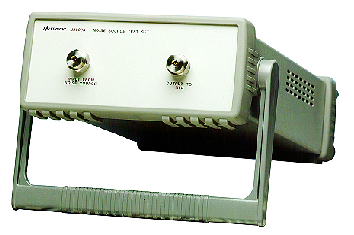
\includegraphics[height=6cm]{./Imagenes/BancoAtenuadoresAisladoresN2002.pdf}
	\caption{Interfaces eléctricas del N2002A}			
	\label{Fig:BancoAtenuadoresAisladoresN2002.pdf}
\end{figure}			

En la medición de figura de ruido de alta precisión la incertidumbre de esta esta fuertemente relacionada a la incertidumbre de la fuente de ruido empleada en la medición. Al conformar un banco de calibración de NS empleando el N2002A, se pueden realizar mediciones de alta precisión en “casa”, lo que evita recurrir a laboratorios especializados	para efectuar esta tarea.

se debe emplear cuando se efectúan mediciones de ENR alta precisión en fuentes de ruido.

El N2002A se inserta en el camino de señal de RF o UW, entre la salida de la fuente de ruido bajo prueba y la entrada	del NFA. La función de este es de proveer aislamiento entre la fuente de ruido y el NFA con el fin de minimizar el	coeficiente de reflexión. Las reflexiones entre el DUT y la fuente de ruido causan incertidumbre en la potencia de ruido que emerge de la fuente; la medición entonces no se refiere a la impedancia de 50 Ohms deseados, sino a la impedancia actual de la fuente de ruido. Incorporando el N2002A dentro del sistema de calibración se minimiza la interacción entre el DUT y el NFA, minimizando el coeficiente de reflexión y de esta forma la incertidumbre. Esto
permite una calibración más precisa de la fuente de ruido, asegurando precisión, repetibilidad y trazabilidad en las	mediciones ademas de reducir de manera significativa la incertidumbre [2].

En la figura \ref{Fig:VistaInternaN2002} se muestra una vista interna y en la figura \ref{Fig:EstructuraInternaN2002} una vista esquemática de la estructura interna del dispositivo. Se aprecia que este equipo esta conformado por cuatro secciones de atenuadores y una sección de aislador. Los atenuadores o el aislador son conectados o desconectados del camino de señal por medio dos conjuntos de interruptores, etiquetados como A2 y A6 respectivamente en la figura 3. Las señales que controlan estos interruptores provienen del exterior del equipo, son generadas por un dispositivo de la serie 11713 de Agilent / Keysight Technologies, unidad controladora de atenuadores e interruptores. Cada sección de atenuador permite el paso de señal en un rango de frecuencia distinto,
como se indica en la figura 3. El N2002A cubre un rango de frecuencias idéntico al del N8975, va desde \SI{10}{\mega\hertz} MHz hasta \SI{26.5}{\giga\hertz}. 

\begin{figure}[h!]
\begin{minipage}{15cm}					
	\centering
	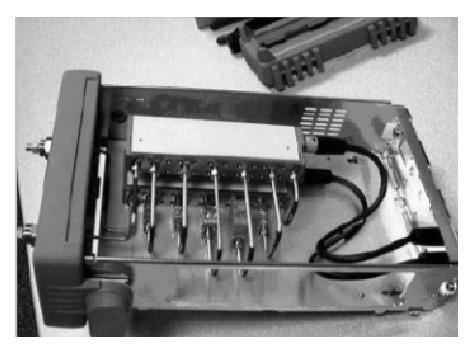
\includegraphics{Imagenes/VistaInternaN2002.png}
	\caption{Esquema de la estructura interna para el N2002S}
	\label{Fig:VistaInternaN2002}
\end{minipage}
\end{figure}			

\begin{figure}[h!]
\begin{minipage}{15cm}					
	\centering
	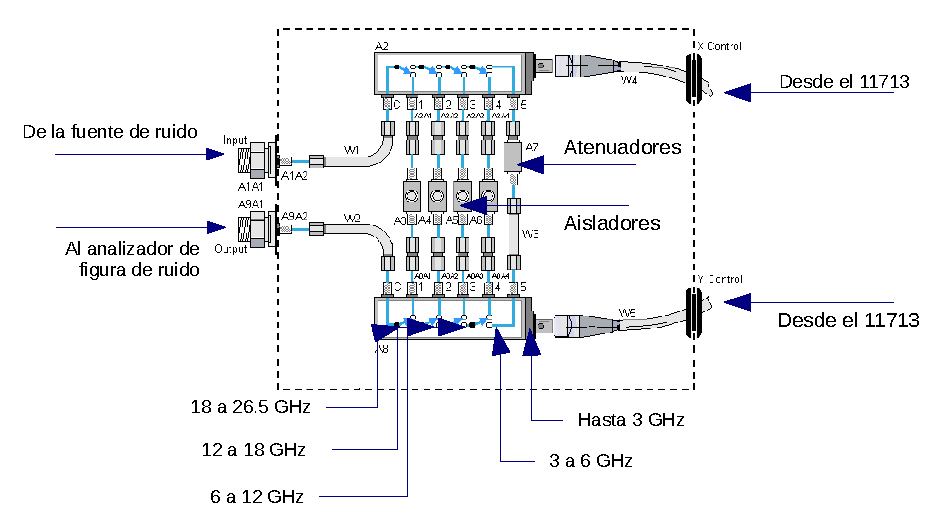
\includegraphics{Imagenes/EstructuraInternaN2002.png}
	\caption{Esquema de la estructura interna para el N2002S}
	\label{Fig:EstructuraInternaN2002}
\end{minipage}
\end{figure}	

\begin{flushleft}
\tablefirsthead{}
\tablehead{}
\tabletail{}
\tablelasttail{}
\begin{supertabular}{|m{4.4570003cm}|m{4.88cm}|}
	\hline
	\multicolumn{2}{|m{9.537cm}|}{\centering Tabla}\\\hline
	\centering A1 &
	\centering\arraybslash Aislador 18 GHz – 26,5 GHz\\\hline
	\centering A2 &
	\centering\arraybslash Aislador 12 GHz – 18 GHz\\\hline
	\centering A3 &
	\centering\arraybslash Aislador 6 GHz – 12 GHz\\\hline
	\centering A4 &
	\centering\arraybslash Aislador 3 GHz – 6 GHz\\\hline
	\centering A5 &
	\centering\arraybslash Atenuador de 3 dB\\\hline
\end{supertabular}
\end{flushleft}

\begin{figure}[h!]
	\centering
	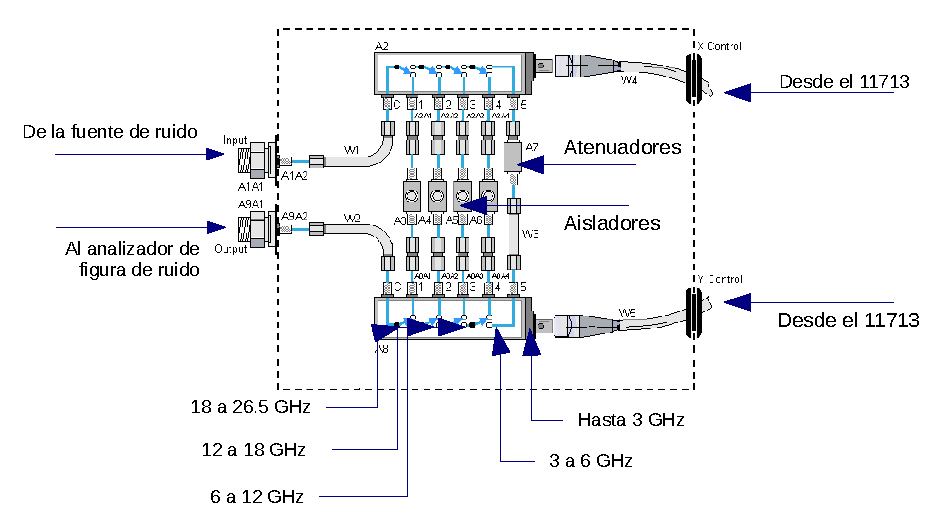
\includegraphics[width=16cm]{./Imagenes/EsquemaEstructuraInternaN2002.pdf}
	\caption{Esquema de la estructura interna del N2002A}			
	\label{Fig:EsquemaEstructuraInternaN2002}
\end{figure}

\begin{table}[h!]
	\centering
	\begin{tabular}{cccc}
		\toprule
		A1 & Aislador 18 \si{\giga\hertz} – 26,5 \si{\giga\hertz} \\
		\midrule
		A2 & Aislador 12 \si{\giga\hertz} – 18 \si{\giga\hertz} \\
		\midrule
		A3 & Aislador 6 \si{\giga\hertz} – 12 \si{\giga\hertz} \\
		\midrule
		A4 & Aislador 3 \si{\giga\hertz} – 6 \si{\giga\hertz} \\		
		\midrule
		A5 & Atenuador 3 \si{\decibel} \\				
		\bottomrule
	\end{tabular}
	\caption{Rangos de ENR nominal para fuentes de ruido serie N4000}
	\label{Tab:RangosFuentesRuido}
\end{table}


\begin{figure}[h!]
	\centering
	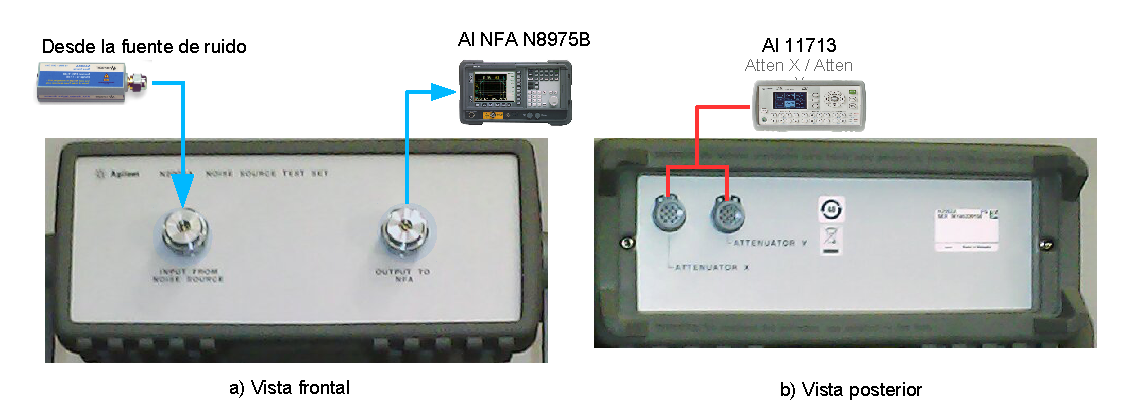
\includegraphics[width=16cm]{./Imagenes/InterfacesElectricasN2002.pdf}
	\caption{Esquema de la estructura interna del N2002A}			
	\label{Fig:InterfacesElectricasN2002}
\end{figure}



El N2002A no posee fuente de poder interna ni tampoco realiza mediciones. No dispone de interfaz de usuario, este equipo debe ser comandado por medio de un dispositivo de la serie 11713. EL 11713 brinda la interfaz de usuario necesaria, en	éste el usuario realiza la selección del rango de frecuencia sobre el cual N2002A debe permitir el paso.		

El N2002A cuenta únicamente con interfaces eléctricas dispuestas en el panel frontal y posterior del equipo (figura \ref{Fig:InterfacesElectricasN2002}). La interfaz para señal de RF / UW esta dispuesta en el panel frontal (figura	\ref{Fig:InterfacesElectricasN2002}a) y posee dos conectores, un conector es la entrada de señal en el cual se conecta la fuente de	ruido (izquierda) y el otro conector es la salida filtrada o atenuada la cual se conecta a la entrada de señal del NFA (derecha). En en el panel posterior se encuentra la interfaz para señales de control (figura \ref{Fig:InterfacesElectricasN2002}b), en esta se encuentran dos conectores para las señales generadas por un dispositivo de la serie 11713.			

\begin{figure}[h!]
	\centering
	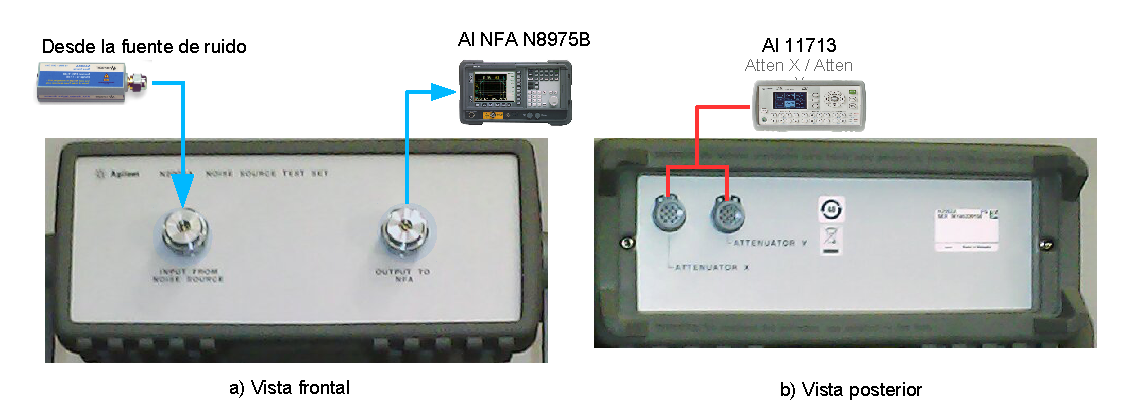
\includegraphics[width=18cm]{Imagenes/InterfacesElectricasN2002.png}
	\caption{Interfaces eléctricas del N2002A}			
	\label{Fig:InterfacesElectricasN2002}
\end{figure}

Según recomendación de Agilent, se debe usar el N2002A en conjunto con el Agilent N8975A (NFA) como equipo básico fundamental para calibración de fuente de ruido. N2002A es un equipo para calibrar fuentes de ruido “en casa” [3.3]. El objetivo es calibrar fuentes de ruido a estándar trazables.

Permite calibrar de manera rápida, repetible con niveles mínimos de incertidumbre. Este equipo es necesario cuando se	realizan pruebas de ENR sobre una fuente de ruido. Asegura resultados de calibración precisos, incrementa la confianza en la medición, permite el desarrollo de DUTs con especificaciones más exigentes. Entrega resultados trazables a 	estándares nacionales.

El proceso de calibración consiste en comparar el desempeño de forma trazable de una fuente de ruido en relación al desempeño de otra fuente de ruido, que se toma como estándar de calibración, o contra las especificaciones del fabricante. Para ello se realizan \ dos pruebas de verificación de desempeño: 

\begin{itemize}
\item Medición de la razón de ruido excedente (ENR).
\item Medición del coeficiente de reflexión complejo (magnitud y fase). 
\end{itemize}

Si la fuente de ruido falla cualquiera de estas pruebas es indicador que requiere reparación o ajuste.

El sistema de calibración de Agilent permite verificas las fuentes de ruido Agilent de la serie 346 (346A, 346B, 346C) y las fuentes de ruido inteligentes de la serie Agilent N4000A (N4000A, N4001A, N4002A). Este proceso de calibración permite calibrar fuentes de ruido entre \SI{10.0}{\mega\hertz} y \SI{26.5}{\mega\hertz}. 

En la figura \ref{Fig:InstrumentacionCalibracion} se muestra la instrumentación propuesta por Agilent \cite{AGI03} para la medida de coeficiente de reflexión (figura \ref{Fig:InstrumentacionCalibracion}a) y para la medida del ENR (figura \ref{Fig:InstrumentacionCalibracion}b).		

\begin{figure}[h!]
\centering
\begin{minipage}{19.011cm}
	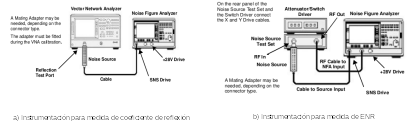
\includegraphics{Imagenes/InstrumentacionCalibracionFuentesRuido.png}
	\caption{ Instrumentación para calibración de fuentes de ruido \cite{AGI03}}
	\label{Fig:InstrumentacionCalibracion}
\end{minipage}
\end{figure}		

\begin{center}
\tablefirsthead{}
\tablehead{}
\tabletail{}
\tablelasttail{}
\begin{supertabular}{|m{9.09cm}|m{7.9370003cm}|}
	\hline
	\multicolumn{2}{|m{17.227cm}|}{Equipo necesario para calibración de NS}\\
	\hline
	Coeficiente de reflexión &	ENR	\\
	\hline
	\begin{itemize}
		\item[] Analizador de Red que cubra el rango 10MHz a 26.5GHz (VNA) 8753ES o 8753ET , 8722Es o 8722ET
	\end{itemize}
	&
	Analizador de figura de ruido N8975A\\
	\hline
	\begin{itemize}
		\item[] N8975A NFA.
	\end{itemize}
	&
	\begin{itemize}
		\item[] N2002A Conjunto para probar fuentes de ruido.
	\end{itemize} \\
	\hline
	\begin{itemize}
		\item[] Kit de calibración apropiado para VNA
	\end{itemize}
	&
	\begin{itemize}
		\item[] 11713A.
	\end{itemize} \\
	\hline
	\begin{itemize}
		\item[] Agilent 11713A
	\end{itemize}
	&
	\begin{itemize}
		\item[] Fuente de ruido de referencia estándar.
	\end{itemize} \\
	\hline
	\begin{itemize}
		\item[] Cable Viking para conexión 11713A
	\end{itemize} \\
	\hline
\end{supertabular}
\end{center}

\subsection{Descripción de las pruebas de verificación [1.28]}
\subsubsection{Medición de ENR [1.28]}
La prueba de ENR consiste en comparar los resultados de la prueba sobre una fuente de ruido bajo prueba (DUT) contra los	resultados de una prueba sobre una fuente de ruido referencia estándar. La referencia estándar es una fuente de ruido calibrada con valores conocidos de ENR. Las medidas se llevan a cabo tanto en la fuente de ruido DUT asi como en la fuente de ruido referencia estándar. Los valores de ENR del DUT se derivan de estos resultados. 

Los resultados de esta prueba permiten asegurar si la fuente de ruido cumple con las especificaciones de calibración del fabricante. La precisión de la medidas para el DUT es altamente dependiente de la exactitud de la calibración de la referencia estándar. Se debe usar, según Agilent, una referencia estándar que haya sido calibrada por un laboratorio especializado.

Las pruebas deben realizarse dentro de la temperatura ambiente de 296 ± 1K (23 ± 1) °C.

Las fuentes de ruido requieren calibración periódica del desempeño operacional. En condiciones de uso normal y ambientales, se calibra la NS cada 12 meses [1.27].

\subsubsection{Resumen del procedimiento de medición de ENR [1.29] [1.39].}
Se emplea la instrumentación indicada en la figura \ref{seq:refDrawing4}b. Se inicia el proceso al encender los equipos y permitir que calienten por una hora. Se debe permitir que las fuentes de ruido se estabilicen a la temperatura	ambiente. No se deben usar las fuentes de ruido una hora antes de realizar las mediciones.
	
Se deben cargar los datos de ENR de la fuente de ruido referencia estándar en el analizador de figura de ruido. Estos datos los proporciona el fabricante de la NS ya sea en formato digital o físico. SI se usa una fuente de ruido inteligente (SNS), el NFA puede cargar los datos de ENR que se encuentran en la memoria de la SNS de forma automática, si el NFA esta habilitado.

La secuencia de pasos para la medición emplea las tabla \ref{seq:refDrawing5}a para registro de resultados

\begin{itemize}
\item Los valores de ENR de la referencia estándar (ENR1) son conocidos, ingresar estos valores en la columna ENR1 de la
tabla 1.
\item Se conecta el equipo de prueba como indica la figura \ref{seq:refDrawing4}b.. Conectar la fuente de ruido de
referencia, asegurando que el conector RF de esta NS es del mismo tipo que el conector de la NS DUT]. Ajustar los
interruptores del 11713, para el canal de frecuencia requerido, por ejemplo interruptores 9 y 0 ON para medir entre
10MHz y 3.0GHz. 
\item Establecer el equipo para realizar la medida del primer punto de frecuencia. 
\item Medir el factor Y lineal de la NS referencia estándar.
\item Anotar este valor en la tabla , bajo la columna Y1.
\item Establecer el equipo para medir el siguiente punto de frecuencia, repetir el procedimiento hasta que todos los
puntos de medición estén completos.
\item Remover la referencia estándar de la entrada del N2002A y la NS DUT.
\item Establecer el equipo para medir el primer punto de frecuencia.
\item Medir el factor Y lineal en la NS DUT.
\item Anotar en las tablas de registro el resultado bajo la columna Y2.
\item Repetir el procedimiento para todos los puntos a medir.
\item Con los resultados obtenidos, introducirlos en las ecuaciones y calcular con ellas el ENR y los valores de
incertidumbre.
\end{itemize}

Conectar cables Viking de la parte posterior del 11713A a la parte posterior del N2002A. Conectar Atten X del 11713A al Attenuator X del N2002A. Conectar Atten Y del 11713A al Attenuator Y del N2002A.

Proceso de Calibración [1.26]	
SI la fuente de ruido falla cualquiera de estas pruebas de desempeño, la NS requiere reparación.

Aparte de la calibración en puntos cardinales de frecuencia, se puede realizar la calibración en otros puntos. El máximo de puntos frecuencia-ENR es de 81.
	
Tabla de VSWR típico en [1.19]

Agilent N2002A empleado cuando se requiere realizar pruebas de Razón de Ruido en Exceso (ENR) sobre una fuente de ruido [1.14]. 

\subsubsection{Ecuaciones}
\emph{ENR}
$\mathit{ENR}_2=10\log (\frac{(Y_2-1)(T_0\frac{10^{\frac{\mathit{ENR}_1}{10}}}{Y_1-1})}{T_0})$ (1)

\emph{text}{Incertidumbre}
$U_C\mathit{ENR}_2=\sqrt{(U_C\mathit{ENR}_1)^2+(U_C\mathit{Sys})^2}$ (2)

donde

TO = 290 K.

ENR1 = Valor de ENR de la fuente de ruido de referencia en cada punto de frecuencia.

ENR2 = Valor calculado de ENR de la fuente de ruido DUT en cada punto de frecuencia.

Y1 = Valor medido del factor Y de la fuente de ruido de referencia en cada punto de frecuencia.

Y2 = Valor medido del factor Y de la fuente de ruido DUT en cada punto de frecuencia.

UcENR1 = Valor de incertidumbre de ENR de la fuente de ruido de referencia en cada punto de frecuencia.

UcENR2 = Valor calculador para la incertidumbre de ENR de la fuente de ruido de referencia en cada punto de frecuencia.

UcSys = Incertidumbre total del sistema de medición en cada punto de frecuencia.

	
\begin{figure}
\centering
\begin{minipage}{15.983cm}
	[Warning: Draw object ignored]Figura {\refstepcounter{Drawing}\theDrawing\label{seq:refDrawing5}}: Tablas para registro
	de datos, relativos a la medición de ENR
\end{minipage}
\end{figure}
El N2002A es controlado por el 11713A. El 11713A es controlado por el software N2002A Noise Source Demonstration Software \ (No encontrado. Ver en su lugar VEE PRO en KeySight).

Equipo de Prueba Recomendado


Para mediciones de ENR y el coeficiente de reflexión (magnitud \ y fase), equipo listado en las tablas 2-4 y 2-5 del
documento [1].		

\subsection{Medición de coeficiente de reflexión (magnitud y fase) [1.31]}
\subsection{Rango de las mediciones de ENR para fuentes de ruido Agilent}
La medición de ENR sobre la fuente de ruido permite garantizar que esta se encuentre dentro de las especificaciones, por ejemplo dadas por Agilent en la tabla 1.		

\begin{figure}
\centering
\begin{minipage}{5.29cm}
	Tabla 3 [1.30]:				
	Rango de ENR para fuentes de ruido
\end{minipage}
\end{figure}
Automatización del proceso de medición

El software que automatiza el proceso de medición esta escrito dentro de Agilent VEE Pro, el cual parece ser un entorno de ejecución (run time), esta disponible como un archivo VEE Pro o un archivo VEE Pro run time (posiblemente sea un script). 

\begin{itemize}
\item Software listado en [3.8]
\item Agilent VEE Pro
\item Agilent VEE Pro run time (provisto con el N2002A)
\end{itemize}
VEE Pro puede comunicarse a través de GPIB, LAN, USB, RS-232, VXI y LXI.

Para su uso requiere una tarjeta de interfaz GPIB (Agilent o National Instruments).

Sistema de calibración de fuente de ruido Agilent		

El sistema de la figura 1 cuenta con los equipos [2.5]:

\begin{itemize}
\item NFA N8975, opera en un rango de 10MHz a 26.6GHz) (con opción 1D5 la cual es una referencia de frecuencia de alta
estabilidad). 
\item Cuenta con el N2002A conjunto para pruebas con fuente de ruido que puede incluir todos los cables y conectores
necesarios para ejecutar calibración de NS con conectores de 3.5mm y tipo N (opción 001). Incluye el 11713A. 
\item Incluye una fuente de ruido estándar de oro.
\end{itemize}
Características del sistema [2.5]

Entre otras, puede calibrar fuentes de ruido tipo SNS y de la serie 346 de Agilent.

Nota importante de [2.3]

El N2002A conjunto para pruebas con fuente de ruido debe ser usado en un sistema de calibración de fuente de ruido, este
equipo no posee fuente de poder y no realiza mediciones.

\subsection{Equipo complementario al N2002A}
Según [2.4] este equipo cuenta con las fuentes de ruido inteligentes (SNS) Agilent de la serie N4000 y de la serie 346.

\subsection{Prueba de verificación [1.17]}
Por medio de un analizador vectorial de red se verifica el coeficiente sea el que indica la tabla para cada frecuencia.

\begin{flushleft}
\tablefirsthead{}
\tablehead{}
\tabletail{}
\tablelasttail{}
\begin{supertabular}{|m{3.972cm}|m{1.012cm}|m{1.012cm}|m{1.012cm}|m{1.012cm}|m{1.012cm}|m{1.012cm}|m{1.012cm}|m{1.012cm}|m{1.012cm}|m{1.012cm}|}
	\hline
Frecuencia (GHz) & 9 &  10 & 11 & 12 & 13 & 14 & 15 & 16 & 17 &\arraybslash 18	\\
\hline
Limite de ROE típico & 1:1.15 & 1:1.15 & 1:1.15 & 1:1.15 & 1:1.15 & 1:1.15 & 1:1.15 &
1:1.15 & 1:1.15 & \arraybslash 1:1.15	\\
\hline
Combinación botones 11713 & 3 - 7 & 3 - 7 & 3 - 7 & 3 - 7 & 2 - 6 & 2 - 6 & 2 - 6 & 
2 - 6 & 4 - 8 & \arraybslash 4 - 8	\\
\hline
\end{supertabular}
\end{flushleft}

\begin{flushleft}
\tablefirsthead{}
\tablehead{}
\tabletail{}
\tablelasttail{}
\begin{supertabular}{|m{3.972cm}|m{1.012cm}|m{1.012cm}|m{1.012cm}|m{1.012cm}|m{1.012cm}|m{1.012cm}|m{1.012cm}|m{1.012cm}|m{1.012cm}|}
	\hline
	Frecuencia (GHz) & 19 & 20 & 21 & 22 & 23 & 24 & 25 & 26 & \arraybslash 25.5 \\
	\hline
	Limite de ROE típico & 1:1.18 & 1:1.18 & 1:1.18 & 1:1.18 & 1:1.18 & 1:1.18 & 1:1.18 &
	1:1.18 & \arraybslash 1:1.18\\
	\hline
	Combinación botones 11713 &	4 - 8 & 4 - 8 & 4 - 8 & 4 - 8 &	4 - 8 & 4 - 8 &
	4 - 8 & 4 - 8 &	\arraybslash 4 - 8\\
	\hline
\end{supertabular}
\end{flushleft}
[Warning: Draw object ignored]

		\subsection{Controlador de interruptores y atenuadores 11713 (Attenuator Switch Driver)}
Los equipos de la serie 11713 están diseñados para generar las señales de control o conmutación para  bancos de	atenuadores o interruptores electromecánicos para RF y UW, de acuerdo a la selección hecha por el usuario en su panel frontal o en forma de comando enviado de forma remota a este dispositivo a través de un bus GPIB, USB o una red LAN.

Los atenuadores e interruptores coaxiales electromecánicos no disponen de interfaz de usuario, se debe emplear un	equipo de la serie 11713 para que el usuario pueda controlar a estos dispositivos.

El 11713 permite al usuario controlar un banco de interruptores o atenuadores interactuando con su interfaz física en su panel frontal (modo local) y también permite control en modo remoto, el usuario puede enviar comandos a través de un bus GPIB (modelo 11713A), un bus USB o una red LAN (modelos 111713B y 11713C).

Fabricado inicialmente por Agilent Technologies con el modelo 11713A (figura \ref{Fig:Versiones11713}a) actualmente es producido por Keysight Technologies, en dos versiones mejoradas pero que conservan toda la funcionalidad del equipo original de Agilent, en los equipos 11713B (figura \ref{Fig:Versiones11713}b) y 11713C (figura \ref{Fig:Versiones11713}c).

Los equipos de la serie 11713 pueden controlar una amplia gama de modelos de atenuadores o interruptores, en la tabla \ref{Tab:AtenuadoresCompatibles11713} se muestran los modelos compatibles de Agilent. Los interruptores a controlar pueden ser de tipo SPDT, bypass, matrix, transfer y multipuerto.

\begin{figure}
	\centering
	\begin{minipage}{17.552cm}
		\includegraphics{Imagenes/VersionesEquipos11713.png}
		\caption{Versiones para los	equipos de la serie 11713}
		\label{Fig:Versiones11713} 
	\end{minipage}
\end{figure}

\begin{table}
	\centering
	
	\tablefirsthead{}
	\tablehead{}
	\tabletail{}
	\tablelasttail{}
	\begin{supertabular}{|m{8.514cm}|m{8.514cm}|}
		\hline
		\multicolumn{2}{|m{17.227999cm}|}{~}	\\
		\hline
		Modelo de atenuador Agilent & \arraybslash Atenuación\\
		\hline
		8494G,H (33320G,H) & \arraybslash 11 dB, paso 1 dB \\
		\hline
		8495G,H,K (33321 G,H,K) & \arraybslash 70 dB, paso 10 dB \\
		\hline
		8496G,H (33322G,H) & \arraybslash 110 dB, paso 10 dB \\
		\hline
		8497K ( 33323K) & \arraybslash 90 dB, paso 10 dB \\
		\hline
		84904K,L (33324K,L) & \arraybslash 11 dB, paso 1 dB \\
		\hline
		84906K,L ( 33326K,L) & \arraybslash 90 dB, paso 10 dB \\
		\hline
		84907K,L (33327K,L) & \arraybslash 70 dB, paso 10 dB \\
		\hline
		
	\end{supertabular}
	
	\caption{Modelos de atenuadores Agilent compatibles con el 11713}		
	\label{Tab:AtenuadoresCompatibles11713}
	
\end{table}

\begin{table}
	\centering
	
	\tablefirsthead{}
	\tablehead{}
	\tabletail{}
	\tablelasttail{}
	\begin{supertabular}{|m{3.504cm}|m{13.527cm}|}
		\hline
		Tipo de interruptor & \arraybslash Modelos Agilent	\\
		\hline
		SPDT & \arraybslash 8761B, 8762A/B/C/F, 8765A/B/C/D/F, N1810TL, N1810UL	\\
		\hline
		Bypass & \arraybslash 8763A/B/C, 8764A/B/C, N1811TL, N1812UL\\
		\hline Multipuerto & \arraybslash 87104A/B/C, 87204A/B/C, 87106A/B/C, 87206A/B/C, 8766K, 8767K, 8768K, 8769K, 8767M, 8768M, 8769M	\\
		\hline
		Matrix & \arraybslash 87406B, 87606B, \\
		\hline Transfer & \arraybslash 87222C/D/E\\
		\hline	 			
	\end{supertabular}
	\caption{Modelos de interruptores Agilent compatibles con el 11713}
	\label{Tab:InterruptoresCompatibles11713}	
\end{table}		

Los equipos de la serie pueden manejar un numero de atenuadores o interruptores, según el modelos. En \ general, el modelo 11713C puede el doble de atenuadores e interruptores que el modelo 11713B.

Los equipos de la serie 11713 disponen de dos tipos de interfaces, una interfaz de usuario y una interfaz eléctrica. Los	equipos 11713B y 11713C agregan una tercera interfaz de comunicaciones. Estos equipos no presentan una interfaz para señales de RF o UW, no manejan ni realizan mediciones sobre este tipo de señales.

La interfaz de usuario se encuentra en el panel frontal de estos equipos, en el 11713A consiste básicamente en tres	grupos de pulsadores. Los equipos 11713B y el 11713C también disponen de pulsadores en su panel frontal y además	agregan una pantalla LCD a la interfaz de usuario.

\begin{center}
	\tablefirsthead{}
	\tablehead{}
	\tabletail{}
	\tablelasttail{}
	\begin{supertabular}{m{2.352cm}|m{3.598cm}|m{3.598cm}|m{3.592cm}|m{3.287cm}|}
		\hline
		\multicolumn{5}{|m{17.227cm}|}{ Interfaz de usuario en los equipos 11713}	\\
		\hline
		\multicolumn{1}{|m{2.352cm}|}{~} &	~ & 11713A & 11713B & \arraybslash 11713C\\
		\hline
		\multicolumn{1}{|m{2.352cm}|}{ Botones} & { Control de atenuadores X\par}				
		{ (ATTENUATOR X)\par}
		
		(1 al 4) &	 1 banco de 4 botones &  1 banco de 4 botones & { 2 bancos de 4 botones cada uno.\par}
		\\\hline
		~ & { Control de atenuadores Y (ATTENUATOR Y) \par} (5 al 6) & 1 banco de 4 botones.  &
		1 banco de 4 botones &	{ 2 bancos de 4 botones cada uno.\par}
		\\\hhline
		{~----} &{ Control de interruptores \par} (9 y 0) &	 1 banco de 2 botones &	{ 1 banco de 2 botones\par}
		~ &	\arraybslash 2 bancos de dos botones cada uno. \\
		\hhline
		{~----} &  Teclas de flecha & No & Si  & \arraybslash Si\\
		\hhline
		{~----}	& Preset, Config, Save/Recall &	No & Si & \arraybslash Si	\\
		\hhline
		{~----}	\multicolumn{1}{|m{2.352cm}|}{ Pantalla LCD} &	~ & No & Si & \arraybslash Si\\
		\hline
	\end{supertabular}
\end{center}	

El 11713 presenta una interfaz eléctrica la cual entrega señales de control que permiten seleccionar un nivel de	atenuación en los atenuadores o abrir y cerrar un interruptor coaxial. Esta interfaz es accesible por medio del panel trasero de los equipos de la serie 11713, en forma de conectores como se aprecia en la figura 8 un detalle del panel	posterior del 11713B. En este panel se encuentran los conectores con las señales de control para atenuadores e	interruptores coaxiales. 

\begin{center}
	\tablefirsthead{}
	\tablehead{}
	\tabletail{}
	\tablelasttail{}
	\begin{supertabular}{|m{4.157cm}|m{4.157cm}|m{4.157cm}|m{4.157cm}|}
		\hline
		\multicolumn{4}{|m{17.227999cm}|}{ Interfaz eléctrica en los equipos 11713}	\\
		\hline
		~ & 11713A & 11713B & \arraybslash 11713C	\\
		\hline
		{ Control de atenuadores\par}
		(conectores Viking de 12 pines) & 1 par de conectores  & 1 par de conectores &
		\arraybslash 2 pares de conectores \\
		\hline
		{ Control de interruptores coaxiales\par}				
		(jacks banana) &  1 par (A y B) & 1 par (A y B) &	\arraybslash 2 pares	\\
		\hline
		Alimentación DC en los puertos  &	+24 V DC & +24 V DC & \arraybslash +5, +15, +24 V DC, ajustable por usuario	\\
		\hline
		Control TTL & No & No & \arraybslash Si	\\
		\hline
		Máximo de atenuadores programables por pasos &	2 de 4 secciones & 2 de 4 secciones &
		\arraybslash 4	\\
		\hline
		Máximo de interruptores coaxiales & { 2 en los jack banana\par}				
		Hasta 10 SPDT con los conectores Viking & { 2 en los jack banana\par}				
		Hasta 10 SPDT con los conectores Viking & { 4 en los jack banana\par}			
		\arraybslash Hasta 20 SPDT con los conectores Viking\\\hline
	\end{supertabular}
\end{center}

En un banco de atenuadores, como los de Agilent, la cantidad de atenuación que se introduce en el camino de señal es determinada por apertura o cierre de un un conjunto de interruptores electromecánicos, que insertan o retiran atenuadores en el camino de señal. Los interruptores coaxiales también emplean interruptores electromecánicos. Las señales de comando que el 11713 envía a los interruptores electromecánicos es una señal de potencia, de tipo lógico y	referidas a tierra.

Las señales de control para los modelos de atenuadores Agilent se encuentran en los conectores Viking. Existe un par de éstos en los modelos 11713 A y B, etiquetados como ATTEN X y ATTEN Y. El modelo 11713C dispone de dos pares de conectores Viking. Las señales presentes en los conectores Viking también pueden emplearse para el control de interruptores electromecánicos coaxiales.

La conexión entre un equipo de la serie 11713 con un atenuador o un interruptor coaxial se realiza por medio de cables	especiales que se insertan en los conectores que disponen estos equipos. La información sobre modelos de cable de acuerdo al modelo de atenuador o interruptor se ofrece en las hojas de datos en forma de matrices de selección. Los cables de conexión se eligen de acuerdo al numero de opción de los equipos 11713 y de acuerdo al modelo del equipo	atenuador o interruptor, ubicando estos datos en la matriz de selección. La matriz de selección remite a una figura en
donde se indica un esquema con instrucciones para realizar las conexiones entre éstos equipos. 

\begin{figure}
	\centering
	\begin{minipage}{17.157cm}
		\includegraphics{Imagenes/PanelPosterior11713.png}
		\caption{Sección del panel posterior del 11713B}
		\label{Fig:PanelPosterior11713}
	\end{minipage}
\end{figure}

Existe un modelo de cable apropiado para cada modelo de atenuador o interruptor coaxial, pero uno de sus extremos siempre debe poseer un conector Viking hembra si se desean utilizar éstos con un equipo 11713. 

Un conector Viking en el equipo 11713, como se muestra en la figura \ref{Fig:PanelPosterior11713},  posee 12 pines. Los pines 1 y 2 portan la tensión DC para alimentar al periférico. Esta tensión de alimentación DC en los equipos 11713A y	11713B es de valor fijo de +24 V DC, en el 11713C puede ser seleccionada por el usuario a un valor fijo de +5, +15, +24	V DC o ajustada a un valor entre 0 y +24 V DC. Los pines del 3 al 12 llevan las señales de conmutación, las cuales son de tipo lógico. En la figura \ref{Fig:PinoutConectorViking} se muestra un esquema de driver interno en el 11713 para las señales	de control. De esta figura se deduce que las señales de control trabajan en pares, esto es, mientras un pin es llevado a tierra el pin complementario es colocado en alta impedancia. Las señales de control en conjunto con la alimentación DC común permite manejar parejas de interruptores electromecánicos en dos estados, abierto y cerrado, o interruptores electromecánicos simples en los cuales una bobina abre y otra bobina cierra el circuito.		

\begin{figure}
	\centering
	\begin{minipage}{17.268cm}
		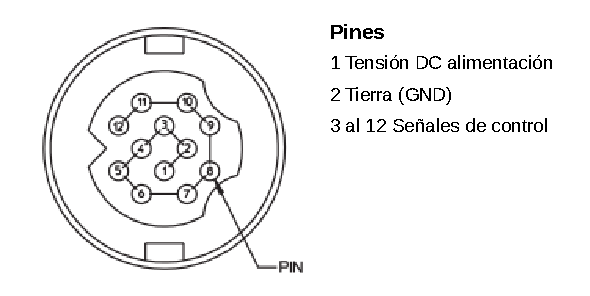
\includegraphics{Imagenes/PinoutConectorViking.png}
		\caption{Disposición de pines en un conector Viking}
		\label{Fig:PinoutConectorViking}
	\end{minipage}
\end{figure}		

\begin{figure}
	\centering
	\begin{minipage}{17.214cm}
		\includegraphics{Imagenes/DriverInternoViking.png} 
		\caption{Diagrama interno generación de señales en conectores Viking}
		\label{Fig:DriverInternoViking}				
	\end{minipage}
\end{figure}

Los conectores banana ubicados en el panel posterior en los equipos 11713 (\ref{Fig:PanelPosterior11713}) están destinados al comando de interruptores electromecánicos coaxiales. Están dispuestos en parejas y etiquetados como A y B. En los modelos 11713A	y 11713B existen dos pares de éstos (S0 y S9) y en el modelo 11713C posee cuatro pares con las etiquetas S0 y S9 (Bank1 y Bank2). En la figura \ref{Fig:DriverInternoBanana} se muestra un diagrama del driver interno para estos puertos. Ambos jacks bananas, A y B, generan una señal de tipo binaria y trabajan de forma complementaria, esto significa que cuando un jack presenta la tensión de tierra (0 V) el jack complementario presenta una tensión DC. Cada grup de conectores S0 y S9 diponen de un jack banana común con un suministro de alimentación DC, para los interruptores que la requieran. Esta tensión de alimentación en los equipos 11713A y 11713B es fija en +24 V DC. En el modelo 11713C esta tensión es puede ser programada por el usuario a un valor fijo de +5, +15 y 25 VDC o ajustada a un valor entre 0 y +24V DC.

\begin{figure}
	\centering
	\begin{minipage}{17.404cm}
		\includegraphics{Imagenes/DriverInternoJacks.png}
		\caption{Diagrama interno generación de señales en un jack banana}
		\label{Fig:DriverInternoBanana}				
	\end{minipage}
\end{figure}

En el sistema para medición de ruido de la \ref{Fig:BancoAtenuadoresAisladores}, un equipo de la serie 11713 se emplea con un doble propósito, servir como interfaz de usuario y controlador del banco de atenuadores N2002. El estado de cada pareja de pines en un conector Viking en el panel posterior de estos equipos esta relacionado en forma directa con el estado del un botón en el panel frontal. En la tabla \ref{Tab:PinesBotones11713} se indica esta relación. Los botones en el panel frontal ubicados en	la sección etiquetado como Attenuator X controlan el estado de los pines ubicados en el conector Viking del panel posterior etiquetado como ATTEN X. Se cumple una relación idéntica para los botones en la sección etiquetada como Attenuator Y del panel frontal y los conectores Viking etiquetados como ATTEN Y del panel posterior. Por ejemplo los pines 5 y 6 en el conector Viking ATTEN X se corresponde al estado del botón 1 en la sección Attenuator X. De la misma forma, los pines 5 y 6 del conector Viking ATTEN Y responden al estado del botón 5 de la sección Attenuator Y.

\begin{table}			
	\raggedright
	\caption{Relacion entre el estado de los pines en el conector Viking y los botones en el panel frontal}
	\label{Tab:PinesBotones11713}
	\begin{tabular}{|m{2.34cm}|m{5.448cm}|}									
		Relación botones panel frontal con los pines en puertos Viking	\\
		\hline
		{ Pines\par} ATTEN X y ATTEN Y & { Controlado por botones \par}	\arraybslash Attenuator X, Attenuator Y	\\
		\hline
		1 & \arraybslash Alimentación \\
		\hline
		2 & \arraybslash Tierra (GND)	\\
		\hline
		5 & { Botón 1 para ATTEN X \par} \arraybslash Botón 5 para ATTEN Y	\\
		\hline
		\multicolumn{1}{|m{2.34cm}}{ 6} & \\	
		\hhline
		{-~} 7 & { Botón 2 para ATTEN X\par} \arraybslash Botón 6 para ATTEN Y	\\
		\hline
		\multicolumn{1}{|m{2.34cm}}{ 8} &	\\
		\hhline
		{-~} 9 & { Botón 3 para ATTEN X \par} \arraybslash Botón 7 para ATTEN Y	\\	
		\hline
		\multicolumn{1}{|m{2.34cm}}{ 10} &	\\	
		\hhline
		{-~}  11 & { Botón 4 para ATTEN X \par}	\arraybslash Botón 8 para ATTEN Y	\\
		\hline
		\multicolumn{1}{|m{2.34cm}}{ 12} &	\\
		\hhline{-~}
	\end{tabular}			
\end{table}	

Los pines en los puertos Viking operan en pareja y de forma complementaria, cuando un pin se encuentra a tierra (GND) su	pareja correspondiente se encuentra en alta impedancia. En la tabla \ref{Tab:RelacionEstadoBotonesViking} se indica la relación que existe entre el estado de los botones en el panel frontal y el estado de los pines en los conectores Viking. Por ejemplo, cuando el botón 1 del panel Attenuator X se encuentra encendido, en el respectivo conector Viking ATTEN X, el pin 5 se encuentra a tierra (GND) mientras que su pin complementario se encuentra en alta impedancia. Cuando el mismo botón se apaga, los pines 5 y 6 intercambian de estado.

\begin{table}
	\centering
	\caption{Relacion entre los estados de los botones en el panel frontal y los pines en los conectores Viking}
	\label{Tab:RelacionEstadoBotonesViking}
	\begin{tabular}{m{1.2179999cm}m{1.2179999cm}m{2.892cm}|m{2.217cm}|m{2.218cm}|}
		
		\multicolumn{5}{m{10.563001cm}}{{ Tabla\stepcounter{Table}{\theTable}\par}					
			Configuración botones y pines puerto Viking}\\\hline
		\multicolumn{2}{|m{2.636cm}|}{{ Botones \par} ATTENUATORS} & Estado del botón &
		\multicolumn{2}{m{4.635cm}|}{{ Estado de los pines puerto \par} ATTEN}	\\
		\hline
		\multicolumn{1}{|m{1.2179999cm}|}{ X } & Y & & Pin & \arraybslash Estado	\\
		\hhline
		{--~--}
		\multicolumn{1}{|m{1.2179999cm}|}{ 1} &
		\multicolumn{1}{m{1.2179999cm}|}{ 5} &
		OFF & 5  &	\arraybslash GND\\	
		\hline	
		&	&	& 6 & \arraybslash Hi Z	\\
		\hhline
		{~~~--} &	& ON & 5 & \arraybslash Hi Z	\\
		\hhline
		{~~---}	&	&	& 6 & \arraybslash GND	\\
		\hhline
		{~~~--}
		\multicolumn{1}{|m{1.2179999cm}|}{ 2} &
		\multicolumn{1}{m{1.2179999cm}|}{ 6} &
		OFF & 7 & \arraybslash GND	\\
		\hline
		& &	& 8 & \arraybslash Hi Z	\\
		\hhline
		{~~~--}
		& & ON & 7 & \arraybslash Hi Z	\\
		\hhline
		{~~---}	& &	& 8 & \arraybslash GND	\\
		\hhline
		{~~~--}
		\multicolumn{1}{|m{1.2179999cm}|}{ 3} &
		\multicolumn{1}{m{1.2179999cm}|}{ 7} &
		OFF & 9 &	\arraybslash GND	\\
		\hline
		&	&	& 10 & \arraybslash Hi Z	\\
		\hhline
		{~~~--}	&	& ON & 9 &	\arraybslash Hi Z	\\	
		\hhline
		{~~---}	&	&	& 10 &	\arraybslash GND	\\
		\hhline
		{~~---}
		\multicolumn{1}{|m{1.2179999cm}|}{ 4} &
		\multicolumn{1}{m{1.2179999cm}|}{ 8} &
		OFF & 11 &	\arraybslash GND	\\
		\hline
		&	&	& 12 & \arraybslash Hi Z	\\
		\hhline
		{~~~--} &	& ON & 11 &	\arraybslash Hi Z	\\
		\hhline
		{~~---} & & & 12 &	\arraybslash GND	\\
		\hhline
		{~~~--}
	\end{tabular}			
\end{table}	

Los jack banana presentes en el panel posterior, etiquetados como A y B bajo las secciones S9 y S0, también operan por parejas, su estado es complementario y es función del estado presente en los botones del panel frontal, etiquetados como S9 y S0. La tabla \ref{seq:refTable3} resume la relación que existe entre los botones S9 y S0 con los niveles de	tensión presentes en los jack banana A y B de las secciones S9 y S0. Por ejemplo, de la tabla \ref{seq:refTable3} se	observa que cuando el botón S9 esta encendido (ON), en la sección S9 del panel posterior el estado el jack banana A
\ se encuentra puesto a tierra (0 V) mientras que el jack banana B presenta una tensión positiva DC (+24 V en el 11713 A). Si ahora el botón S9 se apaga (OFF), los jacks banana A y B de la sección S9 intercambian de estado.

\begin{table}
	\centering
	\begin{tabular}{m{2.0cm}|m{2.5019999cm}|m{1.6099999cm}|m{1.694cm}|m{1.583cm}|}
		
		\multicolumn{5}{m{10.189cm}}{{\centering Tabla {\refstepcounter{Table}\theTable\label{seq:refTable3}}\par}
			
			\centering Relación entre los botones S9 y S0 en el panel frontal y los jacks banana en el panel posterior}\\\hline
		\multicolumn{1}{|m{2.0cm}|}{\centering Interruptor coaxial} &
		\centering Estado botones S9 y S0 &
		\multicolumn{3}{m{5.287cm}|}{\centering Tensión en el jack banana panel posterior}\\\hline
		&
		&
		\centering Jack &
		\centering A &
		\centering\arraybslash B\\\hhline{~~---}
		\multicolumn{1}{|m{2.0cm}|}{\centering S9} &
		\centering OFF &
		\centering S9  &
		\centering +V DC &
		\centering\arraybslash GND \\\hline
		&
		\centering ON &
		\centering S9 &
		\centering GND  &
		\centering\arraybslash +V DC\\\hhline{~----}
		\multicolumn{1}{|m{2.0cm}|}{\centering S0} &
		\centering OFF &
		\centering S0  &
		\centering + V DC &
		\centering\arraybslash GND\\\hline
		&
		\centering ON &
		\centering S0  &
		\centering GND  &
		\centering\arraybslash +V DC\\\hhline{~----}\end{tabular}
	
\end{table}

En el sistema para medición de figura de ruido, el banco de atenuadores N2002 permite el paso de ciertos intervalos de
frecuencia de acuerdo al estado de los botones en el panel frontal de un equipo de la serie 11713. \ \ En la tabla
\ref{seq:refTable4} se muestran los rangos de frecuencia de las señales para las cuales el N2002 permite el paso en
función del estado de los botones en las secciones Attenuator X y Attenuator Y del panel frontal de un 11713. De esta
tabla, cuando los interruptores S9 y S0 están presionados, el N2002 admite el paso de señales cuyas frecuencias se
encuentre entre 10 MHz y 3 GHz. Cuando los botones 1 y 5 de las secciones respectivas Attenuator X y \ Attenuator Y del
panel frontal están presionados, el N2002 admite el paso de señales con frecuencias comprendidas entre 3 GHz y 6 GHz.

\begin{table}
	\raggedright
	\begin{tabular}{|m{3.587cm}|m{1.163cm}|m{1.163cm}|m{1.163cm}|m{1.163cm}|m{1.163cm}|m{1.163cm}|m{1.163cm}|m{1.163cm}|m{1.163cm}|m{1.163cm}|}
		
		\multicolumn{11}{m{17.217001cm}}{{\centering Tabla {\refstepcounter{Table}\theTable\label{seq:refTable4}}\par}
			
			\centering Relación entre los rangos de frecuencia de paso de banda en el N2002 y la combinación de botones en un equipo
			11713}\\\hline
		\centering Rango de frecuencia (MHz) &
		\multicolumn{8}{m{10.704cm}|}{\centering Atenuadores} &
		\multicolumn{2}{m{2.526cm}|}{\centering Interruptores}\\\hline
		&
		\multicolumn{4}{m{5.2520003cm}|}{\centering Attenuator X} &
		\multicolumn{4}{m{5.2520003cm}}{\centering Attenuator Y} &
		&
		\\\hhline{~--------~~}
		&
		\centering 1 &
		\centering 2 &
		\centering 3 &
		\centering 4 &
		\centering 5 &
		\centering 6 &
		\centering 7 &
		\centering 8 &
		\centering S9 &
		\centering\arraybslash S0\\\hhline{~----------}
		\centering 10 a {\textless} 3000 &
		~
		&
		~
		&
		~
		&
		~
		&
		~
		&
		~
		&
		~
		&
		~
		&
		\centering X &
		\centering\arraybslash X\\\hline
		\centering 3000 a 6000 &
		\centering X &
		~
		&
		~
		&
		~
		&
		\centering X &
		~
		&
		~
		&
		~
		&
		~
		&
		~
		\\\hline
		\centering {\textless} 6000 a 12000 &
		~
		&
		~
		&
		\centering X &
		~
		&
		~
		&
		~
		&
		\centering X &
		~
		&
		~
		&
		~
		\\\hline
		\centering {\textgreater} 12000 a 18000 &
		~
		&
		\centering X &
		~
		&
		~
		&
		~
		&
		\centering X &
		~
		&
		~
		&
		~
		&
		~
		\\\hline
		\centering {\textgreater} 18000 a 26500 &
		~
		&
		~
		&
		~
		&
		\centering X &
		~
		&
		~
		&
		~
		&
		\centering X &
		~
		&
		~
		\\\hline\end{tabular}
	
\end{table}

\bigskip

\begin{center}
	\tablefirsthead{}
	\tablehead{}
	\tabletail{}
	\tablelasttail{}
	\begin{supertabular}{|m{5.0880003cm}|m{8.992001cm}|}
		\multicolumn{2}{m{14.280001cm}}{{\centering Tabla \stepcounter{Table}{\theTable}\par}
			
			\centering Especificaciones para interruptores internos}\\\hline
		\centering Tempo de respuesta  &
		\centering\arraybslash 100 $\mu $s máximo parejas de contactos 1 a 8\\\hline
		&
		\centering\arraybslash 20 ms máximo para pareja de contactos 9 y 0.\\\hhline{~-}
		\centering Tiempo de vida &
		\centering\arraybslash Menos de 2 000 000 conmutaciones a 0.7 A para contactos 9 y 0\\\hline
		\centering Máxima inductancia de carga &
		\centering\arraybslash 500 mH\\\hline
		\centering Máxima capacitancia de carga &
		\centering\arraybslash Menor a 0.01uF para contactos 9 y 0\\\hline
	\end{supertabular}
\end{center}
Interfaces de comunicaciones

\begin{center}
	\tablefirsthead{}
	\tablehead{}
	\tabletail{}
	\tablelasttail{}
	\begin{supertabular}{|m{4.157cm}|m{4.157cm}|m{4.157cm}|m{4.157cm}|}
		\hline
		~
		&
		\centering 11713A &
		\centering 11713B &
		\centering\arraybslash 11713C\\\hline
		\centering GPIB &
		\centering Si &
		\centering Si &
		\centering\arraybslash Si\\\hline
		\centering USB &
		\centering No &
		\centering Si &
		\centering\arraybslash Si\\\hline
		\centering LAN &
		\centering No &
		\centering Si &
		\centering\arraybslash Si\\\hline
	\end{supertabular}
\end{center}

\begin{figure}
	\centering
	\begin{minipage}{17.325cm}
		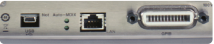
\includegraphics{Imagenes/InterfazComunicaciones11713.png}
		\caption{Puertos en interfaz de comunicaciones}
		\label{Fig:PuertosComunicacionesE5810}
	\end{minipage}
\end{figure}
Control desde panel frontal o remoto, programabilidad de software, interfaz de usuario.

\begin{itemize}
	\item Programación remota desde interfaces \ [1.1]:
	\item GPIB de acuerdo a IEEE 488.2 y IEC65 (compatibilidad con SH0, AH1, T0, TE0, L2, LE0, SR0, RL1, PP0, DC0, DT0, C0).
	\item 10/100 BaseT \ LAN.
	\item USB 2.0.
\end{itemize}
Lenguaje de comandos:

SCPI standard interface commands, compatible hacia atrás con Keysight 11713A.

\subsection{Especificaciones eléctricas}
\subsection{}
\begin{flushleft}
	\tablefirsthead{}
	\tablehead{}
	\tabletail{}
	\tablelasttail{}
	\begin{supertabular}{|m{4.795cm}|m{11.89cm}|}
		\hline
		\multicolumn{2}{|m{16.884998cm}|}{\centering Fuente de alimentación periféricos}\\\hline
		\centering Voltaje &
		{\centering +24V ± 5\%\par}
		
		\centering\arraybslash +24 V ± 2,0 VDC\\\hline
		&
		\centering\arraybslash +5V ± 5\% (Únicamente 11713C)\\\hhline{~-}
		&
		\centering\arraybslash +15V ± 5\% (Únicamente 11713C)\\\hhline{~-}
		\centering Corriente  &
		{\centering 1.7A máxima corriente continua.\par}
		
		{\centering 1.3 A pico máximo por 1 segundo (11713A)\par}
		
		\centering\arraybslash 0.65 A máxima corriente continua (11713A)\\\hline
		&
		\centering\arraybslash Parejas de contactos del 1 al 8, 9, 0 máxima corriente de 0.7A por contacto.\\\hhline{~-}
		&
		~
		\\\hhline{~-}
		\multicolumn{2}{|m{16.884998cm}|}{\centering Fuente de alimentación AC}\\\hline
		\centering Voltaje de linea &
		{\centering 85 a 264 VAC, 47 a 63 Hz (selección automática en 11713B/C)\par}
		
		{\centering 100 o 120 VAC +5\%, -10\% de 48 a 440 Hz (11713A)\par}
		
		\centering\arraybslash 200 o 240 VAC, +5\%, -10\% de 48 a 66 Hz (11713A)\\\hline
		&
		{\centering 100 VA máximo\par}
		
		\centering\arraybslash 80 VA máximo (11713A)\\\hhline{~-}
		\multicolumn{2}{|m{16.884998cm}|}{\centering Especificaciones para interruptores internos}\\\hline
		\centering Tiempo de respuesta  &
		\centering\arraybslash 100 $\mu $s máximo parejas de contactos 1 a 8\\\hline
		&
		\centering\arraybslash 20 ms máximo para pareja de contactos 9 y 0.\\\hhline{~-}
		\centering Tiempo de vida &
		\centering\arraybslash Menos de 2 000 000 conmutaciones para contactos 9 y 0\\\hline
		\centering Máxima inductancia de carga &
		\centering\arraybslash 500 mH\\\hline
		\centering Máxima capacitancia de carga &
		\centering\arraybslash Menor a 0.01uF para contactos 9 y 0\\\hline
	\end{supertabular}
\end{flushleft}


Control remoto de equipo de prueba automatizado de pequeña escala (small scale automated test equipment – ATE). 

Controla hasta 20SPDT interruptores de forma concurrente, o 4 atenuadores programables y 4 interruptores SPDT Y 4
interruptores de microondas.

Con tri-fuente de voltaje integrada , ahorra espacio en rack (unidamente en el 11713C), de 5, 15 y 24V.

El 11713C tiene dos bancos individuales de salidas, con voltajes de comando independientes.

El 11713C posee un driver Fast TTL, con cualquiera de los conectores Viking o en los puertos S0 o S9.

Compatible hacia atrás con el 11713A.

Provee control remoto o desde el panel frontal para atenuadores programables o relés electromecánicos o de estado
solido. Posee UI intuitiva con una variedad de opciones de conmutación, programabilidad de software y características
para control remoto que permiten rápido diseño de pruebas de validación automatizadas.

Programación vía GPIB/USB con instrucciones simples de una linea.

El 11713B y C es un instrumento LXI clase C (LAN eXtensions for Instrumentation – LXI), puede ser controlados de forma
remota a través de una interface web, usada en entornos de alto volumen de producción. 

Posee drivers de instrumentación como IVI-COM que provee compatibilidad de programación con entornos de desarrollo de
apps y soporta estandar de la industria de PC como lo es Component Object Model (COM).

El estandar GPIB soporta automatización a través de programación por mediode scriptsd, \ lo que asegura compatibilidad
con el 11713A.

\subsection{Características 11713B}
Instrumento compatible con GPIB.

Capacidad de manejar de forma concurrente dos atenuadores programables de cuatro secciones, \ dos interruptores
coaxiales para microondas o hasta 10 interruptores SPDT.

De forma opcional posee conectividad USB y LAN.

\subsection[Características 11713C]{Características 11713C}
Instrumento compatible con GPIB, USB, LAN.

Capacidad de manejar hasta cuatro atenuadores programables y cuatro interruptores coaxiales para microondas y hasta 20
interruptores SPDT.

Capacidad de selección de voltaje para drivers de interruptores entre 5 V, 15 V y 24 V admás de voltaje definido por el
usuario. 

\subsection{Usos del 11713}
Según [1.14] \ el equipo puede utilizarse para controlar:

\begin{itemize}
	\item Hasta dos atenuadores programables por pasos de 4 secciones.
	\item Dos interruptores de microondas.
	\item Hasta 10 interruptores SPDT.
\end{itemize}

Tabla Comparativa

Entre los modelos 11713 C y B [2.14].		

\begin{figure}
	\centering
	
\end{figure}

Estos modelos operan con un conjunto de atenuadores, interruptores compatibles y accesorios fabricados por
Agilent-KeySight [2.15].

\subsection[Panel frontal del Keysight 11713B]{Panel frontal del Keysight 11713B}		

\begin{figure}
	\centering
	\begin{minipage}{17.404cm}
		\includegraphics{Imagenes/PanelFrontal11713.png}
		\caption{Panel frontal de un equipo KeySight 11713B}
		\label{Fig:PanelFrontal11713}				
	\end{minipage}
\end{figure}

\begin{center}
	\tablefirsthead{}
	\tablehead{}
	\tabletail{}
	\tablelasttail{}
	\begin{supertabular}{|m{0.881cm}|m{3.9609997cm}|m{11.985001cm}|}
		\hline
		\centering 1 &
		\centering LCD Screen &
		~
		\\\hline
		\centering 2  &
		\centering Botones &
		\centering\arraybslash Botones sin marcas referidos al contenido por el texto de la pantalla\\\hline
		\centering 3 &
		\centering Menu/Enter &
		\centering\arraybslash Presione este boton para activar o desactivar el parámetro con resalte\\\hline
		\centering 4 &
		\centering Preset &
		\centering\arraybslash Presione este boton para establecer en preset el equipo\\\hline
		\centering 5 &
		\centering Config &
		\centering\arraybslash Presione este boton para acceder al menú de configuración. Aquí se establece el tipo de
		atenuador, el voltage de alimentación y la condición TTL.\\\hline
		\centering 6 &
		\centering Save/Recall &
		\centering\arraybslash Presione este botón para almacenar la configuración actual o restaurar configuración previamente
		guardada.\\\hline
		\centering 7 &
		\centering Botones de navegación &
		\centering\arraybslash Los botones con flechas son utilizadors para navegar los parametros mostrados en la pantalla LCD
		o para el cambio de parametros como la dirección GPIB.\\\hline
		\centering 8 &
		\centering Interruptores &
		\centering\arraybslash En modo local, los botonees interruptores 9 y 0 cambian la posición del interruptor coaxial
		conectado a los jck banana ubicados en el panel posterior S9 A/B y S0 A/B respectivamente.\\\hline
		\centering 9 &
		\centering Attenuattor Y &
		\centering\arraybslash En el modo local, los botones 5, 6, 7 y 8 cambian la configuración del la atenuación en el
		atenuador o cambian la posición de los interruptores coaxiales conectados en el conector ATTEN Y en el panel
		posterior.\\\hline
		\centering 10 &
		\centering Attenuator X &
		\centering\arraybslash En el modo local, los botones 1, 2, 3 y 4 cambian la configuración del la atenuación en el
		atenuador o cambian la posición de los interruptores coaxiales conectados en el conector ATTEN X en el panel
		posterior.\\\hline
		\centering 11 &
		\centering On / Standby &
		\centering\arraybslash Presione esta tecla para conmutar entre encendido y standby. Cuando la alimentación es
		suministrada, este LED se ilumina en rojo. Presionar este botón una vez, enciende el equipo y coloca este LED en
		verde.\\\hline
		\centering 12 &
		\centering Local &
		\centering\arraybslash Presione esta tecla para controlar el equipo desde el panel frontal, cuando esta operando via
		interfaz remota.\\\hline
	\end{supertabular}
\end{center}		

\subsection{Panel posterior del KeySIght 11713B.}		

\begin{figure}
	\centering
	\begin{minipage}{17.404cm}
		\includegraphics{Imagenes/PanelPosterior11713.png}
		\caption{Panel posterior de un equipo KeySight 11713B}
		\label{Fig:PanelPosterioral11713}				
	\end{minipage}
\end{figure}

\begin{center}
	\tablefirsthead{}
	\tablehead{}
	\tabletail{}
	\tablelasttail{}
	\begin{supertabular}{|m{0.42300004cm}|m{3.6959999cm}|m{12.87cm}|}
		\hline
		\centering 1 &
		\centering ATTEN X &
		\centering\arraybslash Conector Viking para conexión de un atenuador o interruptores.\\\hline
		\centering 2 &
		\centering ATTEN Y &
		\centering\arraybslash Conector Viking para conexión de un atenuador o interruptores.\\\hline
		\centering 3 &
		\centering S9 A / B &
		\centering\arraybslash Conectores Jack banana para conexión de interruptor coaxial.\\\hline
		\centering 4 &
		\centering 24 VDC COM &
		\centering\arraybslash Conector jack banana que suministra +24VDC para alimentación de los interruptores coaxiales
		conectados en S9 o S0\\\hline
		\centering 5 &
		\centering S0 A / B &
		\centering\arraybslash Conector jack banana para conexión de interruptor coaxial\\\hline
		\centering 6 &
		\centering Receptáculo &
		\centering\arraybslash Conecta el primario del transformador al voltaje de línea \\\hline
		\centering 7 &
		\centering Símbolo de alerta &
		\centering\arraybslash Símbolo de alerta para el usuario\\\hline
		\centering 8 &
		\centering Conector GPIB &
		\centering\arraybslash Conector interfaz para un dispositivo fuente a un dispositivo escucha, usado para operación
		remota.\\\hline
		\centering 9 &
		\centering Conector LAN &
		\centering\arraybslash Interfaz conector para un cable LAN (solo si dispone de la opción LXI)\\\hline
		\centering 10 &
		\centering Conector USB &
		\centering\arraybslash Conector tipo mini{}-B de 5 pines para un cable USB.\\\hline
		\centering 11 &
		\centering Marcas del instrumento &
		~
		\\\hline
	\end{supertabular}
\end{center}

\subsection{}
Importante

El estado de los botones LED indican el pin o cable en el panel trasero que se coloca a tierra, por ejemplo si el botón
3 de ATTENUATOR X esta iluminado, el pin 10 del conector ATTEN X esta a tierra y el pin 9 floata en alta impedancia.

Importante

Corriente de carga máxima en los pines es de 1.7A

Información eléctrica sobre los puertos del panel trasero	

Esquema interno para pines de salida

Se refiere a los botones en el panel frontal marcados como Attenuator X (botones del 1 a 5) y los botones marcados como
Attenuator Y (botones del 5 al 6) \ Cada botón controla una pareja de interruptores basados en transistor en el
interior del equipo, los colectores de estos transistores se conectan a los puertos en el panel trasero marcados como
ATTEN X y ATTEN Y. Usado en el control de atenuadores

Los contactos del puerto trasero ATTEN X y ATTEN Y pueden también manejar hasta 10 relevadores externos, con la
precaución de utilizar diodos de protección en paralelo con la bobina de los mismos, para absorver las sobre tensiones
de conmutación.

Los botones del panel frontal marcados con los números nueve y cero se encargan de controlar la conmutación de los
interruptores ubicados en los banana jack del panel trasero marcados como S9 (A-B) y S0 (A-B). Cuando los botones S9 o
S0 se iluminan, se aplica la tensión del driver (24 V en el 11713A configurable en 11713B/C) al banana jack B y 0V al
jack banana A del conector respectivo en el panel trasero. Cuando los botones S9 o S0 están apagados, la tensión del
driver se aplica al banana jack A y 0 V se aplican al banana jack B de los conectores respectivos del panel trasero.

Los puertos ATTEN X y ATTEN Y también permiten manejar relevadores electromecánicos de acuerdo a la figura 4. La
corriente continua total de carga en loas puerto ATTEN X/ ATENY y S0/S9 debe ser menor de 650 mA.

\begin{figure}
	\centering
	\begin{minipage}{17.491cm}			
		\includegraphics{Imagenes/EsquemaConexionAtenuador.png}
		\caption{Conexión típica para un atenuador programable de 4 secciones}
		\label{Fig:ConexionAtenuador11713}
	\end{minipage}
\end{figure}


\begin{figure}
	\centering
	\begin{minipage}{8.841cm}
		\includegraphics{Imagenes/EsquemaConexionInterruptor.png}
		\caption{Conexión típica para un atenuador programable de 4 secciones}
		\label{Fid:ConexionInterruptor11713}				
	\end{minipage}
\end{figure}

\subsection{\ Puerto GPIB }
Los niveles lógicos del bus son TTL compatibles, presentan lógica negativa: el valor verdadero (1) es representado en el rango de tensión de 0.0 a +0.4 VDC y el valor falso (0) es representado con las tensiones entre +2,5 a +5.0 VDC.

\begin{figure}
	\centering
	\begin{minipage}{10.028cm}
		Figura : Receptáculo GPIB en el panel trasero [2]
	\end{minipage}
\end{figure}		

\subsection{Conexión de atenuadores e interruptores}
Puertos ATTEN X y ATTEN Y

En el panel trasero, los puertos marcados con ATENN X y ATTEN Y poseen conectores macho tipo Viking de 12 pines. Cada
botón en el panel frontal comanda las señales aplicadas a una pareja de pines.

\begin{figure}
	\centering
	\begin{minipage}{11.456cm}			
		\includegraphics{Imagenes/EsquemaConexionCoaxial.png}
		\caption{Conexión de puerto S0 a interruptor coaxial}
		\label{Fig:ConexionCoaxial11713}
	\end{minipage}
\end{figure}


\section{Puente LAN/GPIB para Windows E5810 }

El E5810 actúa como un puente entre una red LAN y equipos que soporten conexión GPIB y/o RS-232. Permite realizar operaciones I/O para obtener mediciones de datos de manera local o remota desde la instrumentación GPIB o RS-232.		
Conexiones de red

EL E5810 puede conectarse a una red de la dos siguientes formas: 

\begin{itemize}
	\item Conexión a una red Empresarial (corporativa).
	\item Conexión a una red Local (LAN aislada).
	\item Conexión directa a una PC.
\end{itemize}
El E5810 puede servir de puente para 14 instrumentos GPIB y para un (1) instrumento RS-232, vía red Ethernet 10BASE-T / 100BASE-TX. El E5810 puede detectar la configuración de red y ajustarse de forma automática a la velocidad apropiada. Este equipo posee un conector RJ-45 en su parte posterior. 

\subsection{Software}
El E5810 incluye Agilent IO libraries Suite, la cual incluye Agilent Virtual Instrument Software Architecture (VISA), VISA COM, Standard Control Library (SICL) y varias utilidades I/O. Este software provee compatibilidad con diferentes fabricantes de software y hardware. Provee una capa de software para operaciones I/O, permite utilizar varios lenguajes como Visual Basic, Visual C++ y Agilent VEE.

El E5810 soporta Dynamic Host Configuration Protocol (DCHP el cual le permite obtener su dirección de IP de forma automática. Por defecto el equipo puede usar DHCP, se puede deshabilitar DHCP y asignar una dirección estática IP al E5810.

El E5810 soporta todas operaciones I/O provistas por VISA, VISA COM, SICL y Agilent VEE. 

Como se muestra en la figura 1, el PC posee las aplicaciones cliente VISA LAN, TCP/IP LAN, necesarias para acceder al E5810. El E5810 posee un servidor LAN además de firmware TCP/IP LAN que le permite actuar como un servidor LAN.

El software cliente realiza conexión con el servidor remoto dentro del E5810, establecida la conexión, el cliente envía peticiones I/O al servidor E5810 a través de la red al servidor E5810, el software instalado en la PC cliente VISA LAN emplea la suite de protocolos TCP/IP LAN para ello. El servidor del E5810 ejecuta estas peticiones de I/O en el instrumento GPIB o RS-232 apropiado.

El E5810 pude servir a múltiples clientes conectados en un momento dado. La cantidad máxima de clientes concurrentes depende del uso de memoria de E5810, la cual esta determinada por el numero de clientes y el numero de sesiones que corren estos clientes. Existe un máximo de 16 clientes accediendo de forma concurrente.

Múltiples instrumentos GPIB se pueden conectar al bus GPIB, pero solo una operación de I/O puede ocurrir en el bus GPIB en un momento dado. Solo se ejecuta una petición de un cliente a la vez, las demás deben esperar hasta que el cliente actual termine. El primer cliente en acceder es el primer cliente servido (cola FIFO).

En caso de que el cliente requiera realizar una secuencia de operaciones I/O que no deban ser interrumpidas, el cliente debe obtener un lock sobre la interfaz GPIB del dispositivo. Completada la operación debe liberar el lock.

\begin{figure}
	\centering
	\begin{minipage}{11.501cm}				
		\includegraphics{Imagenes/EsquemaNetworkStack.png}
		\caption{Network stack}
		\label{Fig:NetworkStack}
	\end{minipage}
\end{figure}

\subsection{Conexiones típicas}

En una conexión Empresarial (corporativa), el E5810 se conecta a la red a través de un router o switch. En esta	configuración, el E5810 es visible en la red Empresarial. En una típica red empresarial consistiría de un Router (Gateway), un servidor corporativo DHCP. El router envía paquetes de información cada host de la red basado en la dirección IP de cada host. La subred esta definida por la mascara de subred. Esta mascara permite identificar a cual subred una dirección IP pertenece. [1.28].

Para que el E5810 pueda operar en una red empresarial requiere de una dirección IP, una mascara de subred (subnet mask) y un puente por defecto (default gateway). 

Si la red soporta DHCP, el E5810 obtiene estos valores del servidor DHCP. SI no soporta DHCP, la dirección IP debe configurarse de forma manual.

\begin{figure}
	\centering
	\begin{minipage}{8.841cm}
		\includegraphics{Imagenes/EsquemaConexionRedE5810-1.png}
		\caption{Configuración de red típica}
		\label{Fig:ConfiguracionRedE5810-1}
	\end{minipage}
\end{figure}

\begin{figure}
	\centering
	\begin{minipage}{8.841cm}
		\includegraphics{Imagenes/EsquemaConexionRedE5810-2.png}
		\caption{Configuración de red típica}
		\label{Fig:ConfiguracionRedE5810-2}
	\end{minipage}
\end{figure}

Para una conexión a red local se emplea un hub o un switch. Puede existir un servidor DHCP. No es visible en la red Empresarial. 

Para una conexión directa desde un PC al E5810, es necesario un cable de crossover, el cual se conecta. desde el puerto LAN del 5810 a el puerto LAN de la tarjeta en la PC. Tampoco es visible en la red empresarial.		

\begin{figure}
	\centering
	\begin{minipage}{8.841cm}
		\includegraphics{Imagenes/EsquemaConexionRedE5810-3.png}
		\caption{Configuración de red típica}
		\label{Fig:ConfiguracionRedE5810-3}
	\end{minipage}
\end{figure}


Panel frontal

Valores de configuración por defecto		

\begin{figure}
	\centering
	\includegraphics{Imagenes/ValoresDefectoE5810.png}
	\caption{Valores por defecto}			
	\label{Fig:ValoresDefectoE5810}
\end{figure}

\subsection{Comunicaciones con el E5810}

El acceso remoto, a través de una red, al E5810 se puede realizar de dos formas:

\begin{itemize}
	\item Por medio del acceso web, a través de un explorador web.
	\item Acceso empleando lenguaje de programación soportado por Agilent IO Libraries Suite.
\end{itemize}

Acceso Web

Empleando un explorador web (como Internet Explorer o Firefox), se accede al E5810 simplemente tecleando en la barra de direcciones la dirección IP o el nombre de host asignado al E5810. Al presionar enter, se mostrará la pantalla de	bienvenida.

A través de esta pantalla se puede configurar los parámetros LAN/GPIB (Configure your LAN/GPIB Gateway) y establecer comunicación con dispositivos GPIB o RS-232.

Acceso empleando un lenguaje de programación.

Se puede programar los instrumentos conectados al E5810 por medio de un lenguaje de programación soportado como C o Visual Basic empleando VISA, VISA COM o SICL. Para ello se deben instalar en la PC las librerías I/O adecuadas,	conocidas como Agilent IO Libraries		

\begin{figure}
	\centering
	\begin{minipage}{11.03cm}
		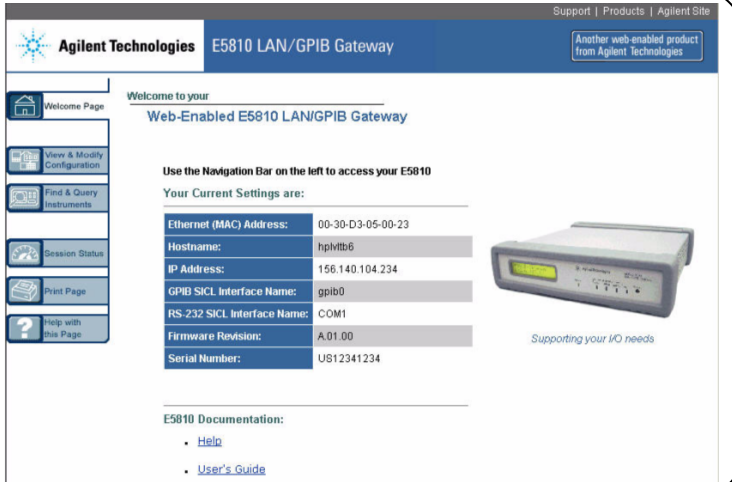
\includegraphics{Imagenes/PantallaBienvenidaE5810.png}
		\caption{Pantalla de bienvenida mostrada en un explorador web (acceso web)}			
		\label{Fig:PantallaBienvenidaE5810}
	\end{minipage}
\end{figure}


Bibliografía

[1] N2002A NOISE SOURCE TEST SET USER'S GUIDE

[2] AGILENT N2002A NOISE SOURCE TEST SET 10MHZ TO 26.5GHZ.

[3] NOISE SOURCE CALIBRATION USING THE AGILENT N8975A NOISE FIGURE ANALYZER AND THE N2002A NOISE SOURCE TEST SET-AGILENT

[4] \ KEYSIGHT N2002A NOISE SOURCE TEST SET-KEYSIGHT	